\chapter{System Model}

\section{系統架構設計}

\subsection{系統分層設計}
本研究設計並實作一套意圖驅動切片編排系統（Intent-Driven Slicing Orchestration System），旨在透過宣告式介面簡化網路切片之管理門檻。如圖 \ref{fig:system_arch} 所示，本系統在視覺架構上劃分為三個主要平面，並依據職能細分為四個管理層級，以符合 3GPP 服務化管理架構（SBMA）之解耦原則。

\begin{figure}[H]
    \centering
    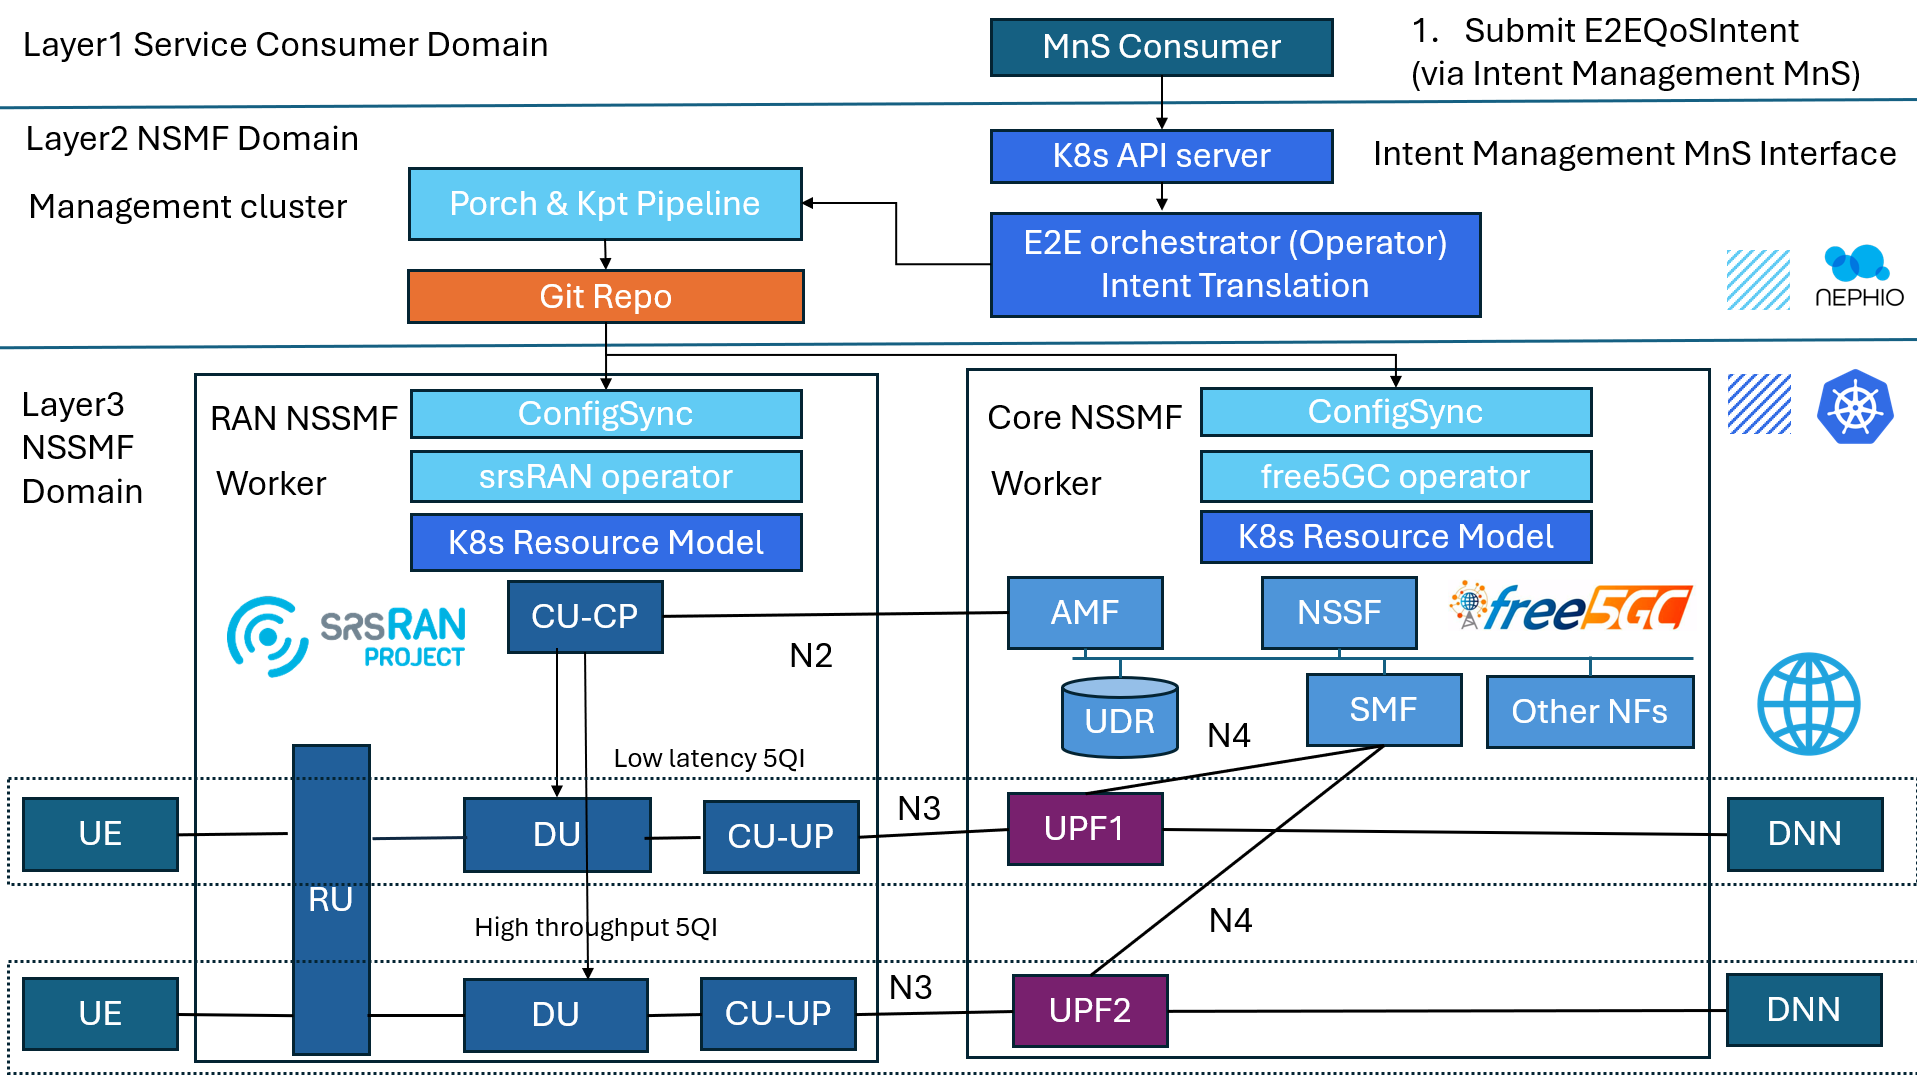
\includegraphics[width=0.95\linewidth]{img/3.1.1-arch.png}
    \caption{本系統之意圖驅動跨網域切片編排架構圖}
    \label{fig:system_arch}
\end{figure}

\begin{enumerate}
    \item \textbf{服務消費者層（Service Consumer Layer）}：對應架構圖中 Layer 1 之 Service Consumer Domain。此層級為管理需求之發起者，扮演 \textbf{MnS Consumer} 之角色。消費者透過 \textbf{Kubernetes API Server} 提供的 \textbf{Intent Management MnS Interface}，下發宣告式之 \texttt{E2EQoSIntent} 自定義資源。使用者僅需根據業務需求定義高階期望指標，例如頻寬期望（\texttt{bandwidth: "high"}）、延遲期望（\texttt{latency: "ultra-low"}）或資源共享策略（\texttt{resourceShare: "Full"}），無需介入底層網域之特定技術配置。

    \item \textbf{意圖編排與協調層（Intent Orchestration Layer）}：對應架構圖 Layer 2 之核心組件。本層級由 \textbf{E2E Orchestrator} 構成，實質承擔 \textbf{NSMF / Intent Handler} 之職能。其負責監聽北向介面之意圖請求，並執行意圖轉譯（Intent Translation），將抽象 SLA 期望精確映射為網域特定參數（如 Core 網域之 5QI 與 RAN 網域之 PRB 比例）。

    \item \textbf{供應與南向介面層（Southbound Interface Layer）}：同樣位於 Layer 2 之管理叢集（Management Cluster）內，負責執行跨網域之編排指令下發。針對 RAN 網域，本系統整合 \textbf{Nephio Porch} 與 \textbf{Kpt Pipeline}，透過 \textbf{Git Repo} 實施配置套件之變更與發布；針對 Core 網域，則透過封裝之 \textbf{REST Client} 執行混合式編排，直接與核心網管理介面進行通訊。

    \item \textbf{網域執行與實施層（Domain Execution Layer）}：對應架構圖 Layer 3 之 NSSMF Domain。此層級負責將編排結果落實於實體網路環境，包含負責無線存取網網域調和之 \textbf{srsran-operator} 與負責核心網網域調和之 \textbf{free5gc-operator}。各 Operator 透過 \textbf{ConfigSync} 監聽期望狀態，並驅動實體網元（如 srsRAN 之 CU/DU 與 free5GC 之各個 NF）執行資源隔離與 QoS 配置。
\end{enumerate}

\subsection{意圖驅動工作流：從 SLA 期望到實體佈署之參數演化}
\label{sec:intent_workflow_trace}

為具體展示本系統如何落實「意圖驅動（Intent-driven）」理念，本節以同時請求 eMBB 與 URLLC 雙切片的情境為例，追蹤意圖參數在系統各層級間的轉譯與流轉過程。在此工作流中，系統將高度抽象的服務層級協議（SLA）期望，逐步解耦並轉化為實體存取網（DU）與核心網的底層配置。

\subsubsection{階段一：意圖下發 (Intent Submission)}
流程始於意圖擁有者（MnS Consumer）下發宣告式資源 \texttt{E2EQoSIntent}。如清單 \ref{lst:input_intent} 所示，該意圖隱蔽了所有 5G 底層技術細節，僅宣告業務端對網路效能的純粹期望。例如，eMBB 業務請求 \texttt{high} 頻寬與部分資源共享（\texttt{Partial}），而 URLLC 業務則嚴格要求 \texttt{ultra-low} 延遲與完全資源隔離（\texttt{Full}）。

\begin{lstlisting}[language=yaml, caption={MnS Consumer 下發之 E2EQoSIntent 完整定義}, label={lst:input_intent}]
apiVersion: e2e.intent.domain/v1alpha1
kind: E2EQoSIntent
metadata:
  name: slices-intent
spec:
  intentGroups:
    - id: embb
      contexts:
        targetUEs: ["208930000000001"]
      expectations:
        sliceType: eMBB
        bandwidth: high
        resourceShare: Partial
    - id: urllc
      contexts:
        targetUEs: ["208930000000002"]
      expectations:
        sliceType: URLLC
        latency: ultra-low
        resourceShare: Full
\end{lstlisting}

\subsubsection{階段二：跨網域意圖轉譯 (Cross-Domain Translation)}
E2E Orchestrator 接收到上述意圖後，其內建的轉譯引擎會依據 3GPP 規範與本地資源池狀態，將 SLA 期望轉譯為具體的網路參數，並回寫至該 CRD 的 \texttt{status} 欄位中（見清單 \ref{lst:translated_params}）。在此階段：
\begin{itemize}
    \item \textbf{Core 參數}：URLLC 的超低延遲期望被精確映射至 \texttt{fiveQI: 85}。
    \item \textbf{RAN 參數}：eMBB 的 \texttt{Partial} 共享被映射為 PRB 比例 0-50\%（優先級 10）；而 URLLC 的 \texttt{Full} 隔離則被賦予最高 100\% 的 PRB 獲取權與極高的排程優先級（Priority 200）。此外，切片識別碼（SD）亦在此階段完成從十六進制（如 0x112233）至十進制（1122867）的系統內碼轉換。
\end{itemize}

\begin{lstlisting}[language=yaml, caption={E2E Orchestrator 轉譯後之參數狀態 (片段)}, label={lst:translated_params}]
status:
  intentGroupStatuses:
    # ... (eMBB 轉譯略) ...
    - id: urllc
      translatedParams:
        coreParams:
          fiveQI: 85
          qfi: 85
        ranParams:
          sst: 1
          sd: 1122867      # 對應 0x112233
          minPrbPolicyRatio: 0
          maxPrbPolicyRatio: 100
          priority: 200
\end{lstlisting}

\subsubsection{階段三：南向配置變更與封裝 (Declarative Package Mutation)}
完成轉譯後，編排器透過 Nephio Porch 對南向存取網域進行配置修改（Mutation）。編排器僅精準替換與切片相關之配置，如清單 \ref{lst:porch_mutation} 所示，\texttt{SrsRANCellConfig} 中的 \texttt{spec.slicing} 陣列被寫入前述的 PRB 與 Priority 參數，而其他實體層參數（如頻段、頻寬）則完整繼承自基礎藍圖（Blueprint）。

\begin{lstlisting}[language=yaml, caption={Porch 修改後之 SrsRANCellConfig 宣告 (片段)}, label={lst:porch_mutation}]
spec:
  # ... (實體層參數沿用 Blueprint) ...
  slicing:
    - sst: 1
      sd: 66051
      schedCfg:
        minPrbPolicyRatio: 0
        maxPrbPolicyRatio: 50
        priority: 10
    - sst: 1
      sd: 1122867
      schedCfg:
        minPrbPolicyRatio: 0
        maxPrbPolicyRatio: 100
        priority: 200
\end{lstlisting}

\subsubsection{階段四：領域實體化與組態生成 (Domain Implementation)}
當宣告式配置透過 GitOps 機制同步至工作負載叢集後，\texttt{srsran-operator} 將攔截此變更。Operator 會遞迴查找 \texttt{NFConfig} 內關聯的所有配置檔，並將 KRM 格式的抽象定義，最終轉化為實體 Distributed Unit (DU) 所需之應用層組態檔。如清單 \ref{lst:final_configmap} 所示，這標誌著從抽象意圖到實體 srsRAN \texttt{gnb-config.yml} 的最後一哩路，確保了切片排程演算法的正確掛載與執行。

\begin{lstlisting}[language=yaml, caption={srsRAN Operator 生成之最終 DU ConfigMap (片段)}, label={lst:final_configmap}]
data:
  gnb-config.yml: |
    # ... (ZMQ 與 F1 介面配置) ...
    cell_cfg:
      # ...
      slicing:
        - sst: 1
          sd: 66051
          sched_cfg:
            min_prb_policy_ratio: 0
            max_prb_policy_ratio: 50
            priority: 10
        - sst: 1
          sd: 1122867
          sched_cfg:
            min_prb_policy_ratio: 0
            max_prb_policy_ratio: 100
            priority: 200
\end{lstlisting}

\section{意圖管理服務介面與端到端編排器實作}
\label{sec:e2e_orchestrator}

本節將深入探討端到端編排器（E2E Orchestrator）的內部架構與實作細節。作為系統中的 \textit{NSMF} 與 \textit{Intent Handler}，該編排器負責介接北向的意圖管理服務，並透過異質的南向介面協調核心網與存取網資源。本節首先定義基於 KRM 的宣告式意圖模型，接著解析跨網域意圖轉譯引擎之演算法，最後分別論述 RAN 與 Core 網域之編排路徑設計，並說明基於狀態回饋的閉環監控機制。

\subsection{宣告式意圖模型設計：\texttt{E2EQoSIntent} CRD 結構與 KRM 規範}
\label{subsec:intent_crd}

為落實 3GPP 所倡導的意圖驅動網路管理（Intent-driven Network Management），本研究開發了名為 \texttt{E2EQoSIntent} 的自定義資源定義（Custom Resource Definition, CRD），作為系統北向的意圖管理服務介面（Intent Management MnS Interface）。

相較於傳統基於 HTTP POST 方法的命令式（Imperative）切片建立 API（例如：\texttt{POST /slice}），本研究採用 Kubernetes 資源模型（Kubernetes Resource Model, KRM）來設計意圖介面，主要基於以下兩項架構優勢：
\begin{enumerate}
    \item \textbf{最終一致性（Eventual Consistency）的保障}：在傳統命令式架構中，若 API 呼叫過程遭遇網路中斷或網元失效，系統狀態極易陷入不一致。透過 KRM 的宣告式（Declarative）設計，MnS Consumer 僅需定義「期望的最終狀態（Desired State）」。底層的 Kubernetes 控制迴圈（Control Loop）將持續不斷地比較「當前狀態（Current State）」與期望狀態，並自動執行調和（Reconciliation），從而在分散式環境中提供強健的容錯與自癒能力。
    \item \textbf{業務意圖與基礎設施的解耦}：\texttt{E2EQoSIntent} 的資料結構被設計為高度抽象的服務層級協議（SLA），意圖擁有者無需具備 5G 底層技術領域知識（如 5QI 映射、PRB 分配算法），即可透過直觀的語意要求網路切片服務。
\end{enumerate}

清單 \ref{lst:input_intent} 展示了 \texttt{E2EQoSIntent} CRD 的 YAML 結構範例。該模型支援單一請求內包含多組意圖（\texttt{intentGroups}），每組意圖透過 \texttt{contexts} 綁定目標用戶設備（\texttt{targetUEs}，以 IMSI 識別），並在 \texttt{expectations} 區塊中宣告高階 SLA 指標，例如切片類型（\texttt{sliceType}）、延遲要求（\texttt{latency}）、頻寬需求（\texttt{bandwidth}）以及資源共享策略（\texttt{resourceShare}）。


\subsection{跨網域意圖轉譯引擎：SLA 指標至 5QI 與 PRB Ratio 之對映演算法}
\label{subsec:intent_translation}

在確立了宣告式意圖模型後，\textit{E2E Orchestrator} 內建的轉譯引擎（Translation Engine）負責將 \texttt{E2EQoSIntent} 中抽象的 SLA 期望（Expectations）解耦，並轉化為底層核心網與存取網可理解且可執行的領域特定參數。此轉譯過程消除了業務端高階需求與底層網路配置間的語意鴻溝（Semantic Gap）。

轉譯引擎之對映演算法分為「核心網（Core）參數轉譯」與「存取網（RAN）參數轉譯」兩個平行維度：

\subsubsection{核心網參數轉譯：基於 3GPP 規範之 5QI 映射}
核心網的轉譯目標為 5G 服務品質識別碼（5G QoS Identifier, 5QI）與對應的 QoS Flow 參數。本演算法嚴格遵循 3GPP TS 23.501 標準中所定義的 QoS 特性進行映射：
\begin{itemize}
    \item \textbf{延遲敏感型業務映射 (URLLC)}：演算法將意圖中的 \texttt{latency} 指標映射至 3GPP 規範的延遲階級。例如，當業務需求宣告為超低延遲（\texttt{ultra-low}）時，引擎會將其精確映射至 \textbf{5QI 85}。在 3GPP 標準中，5QI 85 具備「延遲臨界（Delay Critical）」特性，專為保障嚴苛的錯誤率與延遲限制（Delay Bound）所設計。次之的 \texttt{low} 與 \texttt{medium} 延遲期望，則分別降級映射至 5QI 82 與 5QI 84。
    \item \textbf{頻寬需求型業務映射 (eMBB)}：針對 \texttt{bandwidth} 指標，演算法依據頻寬需求的嚴格程度，對應至 3GPP 中階級不同的 5QI。最高級別的 \texttt{dedicated-high} 映射至具備保證位元速率（GBR）特性的 5QI 4；而 \texttt{high} 與 \texttt{standard} 則分別映射至優先級遞減的非保證位元速率（Non-GBR）類別，即 5QI 6 與 5QI 9。
\end{itemize}

\subsubsection{存取網參數轉譯：S-NSSAI 與無線資源隔離策略}
在存取網端，轉譯重點在於切片識別與無線實體資源區塊（Physical Resource Block, PRB）的調度參數分配：
\begin{itemize}
    \item \textbf{資源隔離比例 (PRB Policy Ratio)}：意圖中的 \texttt{resourceShare} 屬性決定了無線資源的實體隔離程度。若宣告為 \texttt{Full}（如 URLLC），引擎將 \texttt{maxPrbPolicyRatio} 設為 100\%，賦予該切片獲取全局可用頻寬的權限；若宣告為 \texttt{Partial}（如 eMBB），則將 \texttt{maxPrbPolicyRatio} 限制為 50\%，藉此預防單一切片耗盡所有無線資源，落實防飢餓（Starvation Prevention）的隔離目標。
    \item \textbf{排程優先級 (Scheduling Priority)}：為確保在無線資源面臨競爭時，關鍵型業務能被優先排程，演算法為 URLLC 切片配置了極高的 MAC 層排程權重（\texttt{priority: 200}），而一般 eMBB 切片則配置為基礎權重（\texttt{priority: 10}）。
\end{itemize}

\subsection{RAN 子網域編排路徑：基於 Nephio Porch 之宣告式封裝工作流}
\label{subsec:ran_orchestration_path}

在本系統的雙路徑派發架構中，存取網（RAN）子網域採用純宣告式（Declarative）的編排路徑。此路徑為本研究之核心實作貢獻之一，其突破了傳統命令式腳本在分散式環境下容易遭遇的狀態碎片化問題。\textit{E2E Orchestrator} 將 Nephio Porch 作為供應管理服務框架（Provisioning MnS Framework），透過操控 KRM 套件的生命週期，達成切片配置的自動化下發。

\subsubsection{基於狀態機之封裝編排工作流 (Package Orchestration Workflow)}
為了將轉譯後的 PRB Ratio 與 Priority 等參數安全地套用至存取網，\textit{E2E Orchestrator} 內建了 \texttt{PorchClient}，並實作了一套完整的套件變更（Package Mutation）工作流。該工作流嚴格遵循 Porch 狀態機的移轉規範，涵蓋以下自動化步驟：

\begin{enumerate}
    \item \textbf{建立草稿與提取 (Copy \& Pull)}：編排器首先以基礎藍圖（Blueprint）為範本，透過 \texttt{copy} 指令複製出一個全新的套件修訂版（PackageRevision）草稿，並將其拉取（Pull）至記憶體中進行處理。
    \item \textbf{意圖參數注入 (Mutate)}：編排器解析套件內的 \texttt{srscellconfig.yaml} 等資源檔，針對 \texttt{spec.slicing} 陣列進行精準替換。同時，視意圖需求動態修改 \texttt{PLMNConfig}，注入對應的切片識別碼（SST/SD），而未涉及切片的實體層參數則原封不動予以保留。
    \item \textbf{版本推播與提議 (Push \& Propose)}：完成參數替換後，編排器將變更後的套件推播（Push）回 Porch，並將套件狀態推進至 \texttt{Propose}，代表該配置已準備好接受審查。
    \item \textbf{批准發佈 (Approve)}：最終，編排器觸發 \texttt{Approve} 操作，正式發佈該套件。此動作將觸發底層 CISM (Cluster Infrastructure \& Service Management) 代理程式（如 ConfigSync）的同步機制，將配置派發至目標工作負載叢集。
\end{enumerate}

\subsubsection{宣告式編排之學術與工程價值}
透過上述基於 Nephio Porch 的工作流實作，本系統在 RAN 網域的編排上達成了兩項關鍵的雲原生工程特性：
\begin{itemize}
    \item \textbf{具備可追溯性之版本控制 (Version Control)}：所有針對 RAN 切片參數的修改，皆被封裝為不可變的修訂版本（PackageRevision）。這使得網路配置具備了類似軟體程式碼的「單一事實來源（Single Source of Truth, SSOT）」，當意圖發生衝突或配置失效時，系統具備退回（Rollback）至前一穩定版本的基礎能力。
    \item \textbf{確保狀態一致性之原子性變更 (Atomic Mutation)}：在傳統 REST API 連續呼叫的模式下，若中途發生網路異常，極易導致配置僅部分生效的「髒狀態（Dirty State）」。本系統透過 KRM 套件封裝，將 \texttt{SrsRANCellConfig}（PRB 資源劃分）與 \texttt{PLMNConfig}（網路識別廣播）等具備高度相依性的資源打包。當 ConfigSync 進行同步時，這些配置會被視為一個完整的邏輯單元進行套用，確保了變更的「原子性」——意即配置要麼全部生效，要麼全部不生效，從根本上消除了分散式系統中部分配置失敗的隱患。
\end{itemize}

\subsection{核心網子網域編排路徑：基於 REST API 之混合式異質整合機制}
\label{subsec:core_orchestration_path}

在本系統的架構設計中，核心網（Core Network）子網域採用「混合式編排（Hybrid Orchestration）」路徑。此設計不同於存取網（RAN）所採用的純宣告式套件編排，其核心考量在於現有開源核心網實作的功能限制，以及 5G QoS 機制的實施邏輯。

\subsubsection{異質網域編排之實作困境與限制}
在存取網端，如 \textit{srsRAN} 等實作允許透過修改網元組態檔（如 \texttt{cell\_cfg.slicing}）來定義特定切片的資源優先級與 PRB 比例。然而，鑑於現有開源核心網實作（如 \textit{free5GC}），其網路功能（NF）如 SMF 或 UPF 並不具備可供動態調整切片優先級的組態參數。核心網對切片服務品質（QoS）的控制，實質上是透過用戶設備（UE）的註冊資訊與服務合約（Subscription Data）進行綁定。

意圖模型中所定義的 \textit{5QI} 參數，必須透過核心網的註冊機制注入 UE 上下文（UE Context），方能於 PDU 會話建立過程中將 QoS 需求傳遞至存取網，使 RAN 識別該 UE 所屬之切片特性。因此，\textit{E2E Orchestrator} 無法如同處理 RAN 網域般，單純透過 \textit{Nephio Porch} 修改 SMF/UPF 的宣告式組態來達成意圖。

\subsubsection{混合式編排架構之實施}
為了克服上述限制，本系統採用「混合式編排」架構，其核心設計邏輯在於：在維持編排器北向介面（Intent Management MnS Interface）宣告式特性的同時，透過封裝 \textit{REST Client} 確保對異質網域之相容性。

具體實作上，\textit{E2E Orchestrator} 內建了 \texttt{Free5GCClient} 模組，將轉譯後的 5QI、S-NSSAI 與目標 IMSI 封裝為核心網可理解之 REST 指令：
\begin{enumerate}
    \item \textbf{動態用戶註冊}：針對 \texttt{E2EQoSIntent} 中定義的每一組 \texttt{targetUEs}，編排器透過 \texttt{RegisterSubscriber()} 介面自動於核心網建立對應用戶。
    \item \textbf{QoS 參數注入}：若用戶已存在，編排器則調用 \texttt{UpdateSubscriberQoS()}，將意圖轉譯所得之 5QI、SST 與 SD 參數注入該用戶的會話管理訂閱資料（Session Management Subscription Data）中。
\end{enumerate}

\subsection{意圖達成狀態監控：基於 CRD Status 之狀態回饋迴圈}
\label{subsec:intent_monitoring}

意圖驅動編排的核心在於「閉環控制（Closed-loop Control）」邏輯，而有效的狀態回饋是落實閉環控制的前提。在本系統中，\textit{E2E Orchestrator} 利用 Kubernetes CRD 的 \texttt{status} 子資源實作了意圖監控機制，這不僅是用於呈現系統當前狀態，更構成了狀態回饋迴圈（Status Feedback Loop）的觀察基礎。

\subsubsection{意圖達成狀態定義 (Fulfillment State)}
為了使系統具備標準化的評估準則，本研究參考 3GPP TS 28.312 規範，在 \texttt{E2EQoSIntent} 的狀態模型中引入了「達成狀態（Fulfillment State）」指標。編排器會根據各子網域的回報，動態更新以下狀態：
\begin{itemize}
    \item \textbf{FULFILLED}：代表 RAN 與 Core 網域均已正確套用轉譯參數，且底層資源已成功實體化。
    \item \textbf{NOT\_FULFILLED}：代表意圖剛下發或轉譯、派發過程中遭遇錯誤（如 REST API 連線失敗或 Porch 套件衝突）。
    \item \textbf{DEGRADED}：當系統偵測到實體資源狀態（如 Pod 運行狀態）偏離預期，但配置尚未失效時標註。
\end{itemize}

\subsubsection{多維度狀態回饋結構}
如清單 \ref{lst:intent_status} 所示，系統的 \texttt{status} 欄位被設計為階層式結構，以確保監控的可追溯性：
\begin{enumerate}
    \item \textbf{處理階段 (Phase)}：追蹤編排器的處理進度（如 \texttt{Processing} 或 \texttt{Applied}）。
    \item \textbf{觀察世代 (Observed Generation)}：紀錄編排器最後一次處理的意圖版本，結合 Kubernetes 的 \texttt{metadata.generation} 機制，確保編排器能精確偵測到意圖的任何微小變更並觸發重新調和。
    \item \textbf{網域特定狀態 (Domain Status)}：細分核心網（Core）與存取網（RAN）的實施狀態。例如，核心網狀態會反映 \textit{free5GC} 用戶註冊是否成功；存取網狀態則反映 \textit{Nephio} 套件是否完成 Approve 流程。
    \item \textbf{達成目標 (Achieved Targets)}：將底層實施結果重新映射回業務語意（如 \texttt{bandwidth: achieved}），為 MnS Consumer 提供直觀的業務達成率報告。
\end{enumerate}

\begin{lstlisting}[language=yaml, caption={\texttt{E2EQoSIntent} 狀態回饋與監控資訊結構 (範例)}, label={lst:intent_status}]
status:
  phase: Applied
  fulfillmentState: FULFILLED
  observedGeneration: 1
  intentGroupStatuses:
    - id: embb
      domainStatus:
        coreDomain:
          state: CONFIGURED
          message: "UEs registered with 5QI=6"
        ranDomain:
          state: CONFIGURED
          message: "Slice configured: SST=1, SD=66051"
      achievedTargets:
        bandwidth: achieved
        latency: not_applicable
\end{lstlisting}

\subsubsection{基於 Reconciliation 的自癒機制}
此狀態回饋機制直接與編排器的 \textit{Reconciler} 連動。當 \texttt{status} 顯示意圖處於 \texttt{NOT\_FULFILLED} 或發生配置漂移（Configuration Drift）時，控制迴圈會自動再次觸發南向派發流程。例如，若核心網用戶註冊因網路抖動失敗，編排器將在下一次調和週期中自動重試 \texttt{RegisterSubscriber} 操作，直至狀態達到「最終一致性」。這種基於 CRD Status 的設計，使系統具備了基礎的配置自癒（Self-healing）能力。